\documentclass[twocolumn, 10pt,a4j]{jsarticle}
\usepackage{amsmath}
\usepackage[dvipdfmx]{graphicx}
\usepackage{url}
% プリアンブル
\title{\vspace{-2.5cm}11. 自然および強制対流熱伝達}
\author{1610581 堀田 大地}
\date{2018/6/28}
\begin{document}
\maketitle{}
\section{目的}
% 目的
  工業製品は適切な温度状態に保たれなければならない.例えば,コンピュータのCPUは
  稼働中に多量の熱を発するため,うまく放熱されない場合には温度が上昇し続けて
  物理的に演算のできない状態に陥る.よって,効率よく放熱処理を施すことは
  必須である.本実験では熱移動の基本形式の一つである対流熱伝達について理解を
  深める.
\section{原理}
% 原理
    {\bf 自然対流熱伝達}\ 空気や水などの流体ないに温度差が生じると熱膨張による密度差に
  より流体に運動が発生する現象を自然対流と呼び,
  静止した空気中に王恩物体を設置すると壁
  近傍に熱せられた空気の層,つまり温度境界層が生じ,浮力によって層内の空気が
  上方に流動して熱を運んで行く伝熱形式である.
    \par{\bf 強制対流熱伝達}\ 外部からの仕事によって発生する流体の運動を強制対流と呼び,
  このときに行われる熱移動である.
  \\[1ex]\par
    物体の壁面温度を$T_{w}[K]$,流体の壁より十分離れた位置における温度を$T_{0}[K]$,
  面積$A[m^{2}]$の物体表面より単位時間当たりに放出される熱量を$Q[W]$,熱伝達率
  を$h[W/(m^{2}K)]$とすると,
  $Q$は(1)で表せられる.また,$h$の値は対流の種類や強さ,流体の種類によって変化する.
  \begin{equation}
    Q = hA(T_{w} - T_{0})
  \end{equation}

  自然対流による熱伝達率はかなり小さいので,自然対流熱伝達によって放熱を
  行う場合には,高温側壁面にフィンを設けて放熱量の増大を測ることが多い.
  まず,フィンの設置によってどの程度$Q$が増加するかを単純な一枚のフィンの
  場合について考察する.
    \par 定常状態の条件下でフィンの根元を$x$軸の原点にとり,任意断面$x$における
  微小区間$dx$に対する熱収支を考慮すると(2)が導かれる.
    \begin{center}
      \begin{equation}
        (d/dx)[kS・dT / dx]dx - hRdx(T - T_{0}) = 0
      \end{equation}
      \begin{flushleft}
        \ \ \ \ $k$ : フィンの熱伝導率\ ($k$=428\ W/(mK) : 銅) \\
        \ \ \ \ $R$ : フィンのタンメンの接触長\ $2 \times (b+L)$ \\
        \ \ \ \ $S$ : フィン断面積\ $b \times K$ \\
        \ \ \ \ $T$ : $x=x$におけるフィン温度 \\
        \ \ \ \ $T_{0}$ : 周囲の空気温度 \\
        \ \ \ \ $h$ : フィン表面の熱伝達率  
      \end{flushleft}
    \end{center}
    \par $k, S, T_{0}, h = const$とすると,(2)はTに関する二階の常微分方程式(3)
    となり,解は,$T=T_{w}\ at\ x = 0$および,$dT/dx = 0\ at\ x = H$なる
    境界条件により(4)となる.
      \begin{equation}
        d^{2}T / dx^{2} - (hR / kS)(T - T_{0})=0
      \end{equation}
      \begin{equation}
        (T - T_{0}) / (T_{w} - T_{0}) = coshB(H - x) / cosh BH
      \end{equation}
      \begin{equation}
        B = (hR / kS)^{1/2}
      \end{equation}
    
    \par (4)で得られた温度分布$T=T(x)$により,一枚のフィンからの放熱量$Q$は(6)
    で与えられる.
    \begin{eqnarray}
      %(6)
      Q &=& \int_H^0 hR(T - T_{0})dx \nonumber \\
        &=& (hRkS)^{1/2} (T_{w} - T_{0})tanh BH
    \end{eqnarray}
      \par また,$Q$は(7)で定義される基盤からフィンに流入する熱量と等しい.
    \begin{eqnarray}
      %(7)
      Q = -kS[dT / dx]_{x=0}
    \end{eqnarray}
      \par 次に,フィンを付けたことによる放熱量の増加分について検討する.
    フィンがない場合(接触面積\ =\ $S$)の放熱量を$Q_{0}$とし,
    フィンを付けた場合(接触面積\ =\ $RH$)の放熱量$Q$との比を
    $\epsilon$とすると(8)が成り立つ.
    \begin{eqnarray}
      %(8)
      \epsilon = Q/Q_{0} = (kR / hS)^{1/2}tanh BH
    \end{eqnarray}

      \par 以上の結果より,$N$枚のフィンによる放熱量$Q_{N}$は
    (6)による$Q$を用いて(9)で与えられる.ただし,$A_{w}$は
    フィンの表面以外での流体との接触面積$PL$であり,
    フィンと空気との接触面積$A_{f}=2HL$に比べて省略できるものと考える.
    ここで(6)と(9)は,$Q_{N}$を大きくするためには,
    フィンの熱伝導率$k$,枚数$N$,高さ$H$を大きくし,
    厚さ$b$を小さくすればよいことを示している.
    \begin{eqnarray}
      Q_{N} = N[hA_{w} (T_{w} - T_{0}) + Q] \cong NQ
    \end{eqnarray}

\section{実験装置および実験方法}
% 3
    \par 銅性基盤の寸法は$40.0 \times 42.0 mm$であり,指定された厚さ$b$,
  ピッチ$P$,高さ$H$および枚数$N$のフィンに対して実験を行なった.
    \par まずフィン基盤を水平に設置し(この状態での回転角$\theta$を0にとった),
  加熱量一定の条件下でフィンを加熱する.フィン基盤の平行温度が$100 - 150 ^\circ C$
  となるように,ヒータの出力を調整してフィン基盤温度の時間的変化を調べる.
  基盤温度の平均値$T_{wm}$と雰囲気の温度$T_{0}$との差が安定するまで測定を行なった.
  次にフィン基盤の回転角$\theta$を$45^\circ$変化させて,
  $\theta = 45^\circ, 90^\circ, 135^\circ, 180^\circ$において同様の測定を
  繰り返した.
    \par 次に,$\theta = 180^\circ$の状態において,逆風機の電源を入れ,
    一定流量の空気を流し自然対流時と同様に$T_{wm}$と$T_{0}$との差が安定するまで
  測定を行なった.
    \par 実験は加熱量一定の条件下行うので,フィン基盤回転角$\theta$がある値での,
  定常状態における基盤平均温度と雰囲気温度との差は(10)を満たす.
    \begin{eqnarray}
      IE = hA_{f}(T_{wm} - T_{0})
    \end{eqnarray}
  よって,フィン表面の平均熱伝達率$h[W/(m^{2}K)]$を(11)より求めることができた.
    \begin{eqnarray}
      h = IE / [A_{f}(T_{wm} - T_{0})]
    \end{eqnarray}
\section{測定事項}
$H=35.0mm,L=40.0mm,b=1.7mm,N=7$が測定結果として得られた.

\section{結果}
% 結果
\begin{enumerate}
  \item $(T_{wm} - T_{0}) \sim tの関係$ \\
    表1,2に示した.
    \begin{table}[]
      \centering
      \caption{$(T_{wm} - T_{0}) \sim tの関係$}
      \label{my-label}
      \footnotesize
      \begin{tabular}{lllll}
      角度 & 時間 & フィンの温度$T_{wm}$ & 外温度$T_{0}$ & $T_{wm}-T_{0}$ \\ \hline
      0&0&68.2&25&43.2 \\
      &1&68.1&25&43.1  \\
      &2&68.2&25.1&43.1  \\
      &3&68.3&25.1&43.2  \\
      &4&68.4&25.1&43.3  \\
      &5&68.5&25.1&43.4  \\
      &6&68.4&25.1&43.3  \\
      &7&68.3&25.2&43.1  \\
      &8&68.5&25.2&43.3  \\
      &9&68.4&25.2&43.2  \\
      &10&68.5&25.2&43.3  \\
      45&11&68.1&25.2&42.9  \\
      &12&68.2&25.3&42.9  \\
      &13&68.3&25.3&43  \\
      &14&68.3&25.4&42.9  \\
      &15&68.3&25.4&42.9  \\
      &16&68.3&25.3&43  \\
      &17&68.3&25.4&42.9  \\
      &18&68.3&25.4&42.9  \\
      &19&68.5&25.4&43.1  \\
      &20&68.5&25.5&43  \\
      &21&68.5&25.5&43  \\
      \end{tabular}
      \end{table}

      \begin{table}[]
        \centering
        \caption{$(T_{wm} - T_{0}) \sim tの関係$}
        \label{my-label}
        \footnotesize
        \begin{tabular}{lllll}
        角度 & 時間 & フィンの温度$T_{wm}$ & 外温度$T_{0}$ & $T_{wm}-T_{0}$ \\ \hline
        90&22&68.3&25.5&42.8  \\
      &23&68&25.5&42.5  \\
      &24&67.7&25.5&42.2  \\
      &25&67.5&25.5&42  \\
      &26&67.3&25.5&41.8  \\
      &27&67.2&25.5&41.7  \\
      &28&67&25.5&41.5  \\
      &29&66.8&25.5&41.3  \\
      &30&66.7&25.5&41.2  \\
      &31&66.6&25.5&41.1  \\
      &32&66.6&25.5&41.1  \\
      135&33&67&25.6&41.4  \\
      &34&67.2&25.6&41.6  \\
      &35&67.4&25.6&41.8  \\
      &36&67.6&25.6&42  \\
      &37&67.7&25.6&42.1  \\
      &38&67.7&25.6&42.1  \\
      &39&67.8&25.6&42.2  \\
      &40&67.9&25.6&42.3  \\
      &41&68.1&25.6&42.5  \\
      &42&68.3&25.6&42.7  \\
      &43&68.3&25.6&42.7  \\
      180&44&68.9&25.6&43.3  \\
      &45&69.1&25.7&43.4  \\
      &46&69.3&25.7&43.6  \\
      &47&69.4&25.8&43.6  \\
      &48&69.6&25.8&43.8  \\
      &49&69.8&25.8&44  \\
      &50&69.9&25.8&44.1  \\
      &51&70&25.8&44.2  \\
      &52&70.2&25.8&44.4  \\
      &53&70.4&25.8&44.6  \\
      &54&70.5&25.8&44.7  \\
      &55&70.7&25.9&44.8  \\
      180,fun&56&70.4&26.1&44.3  \\
      &57&70.2&26.3&43.9  \\
      &58&70.2&26.4&43.8  \\
      &59&70.6&26.5&44.1  \\
      &60&70&26.5&43.5  \\
      &61&69.6&26.6&43  \\
      &62&70&26.6&43.4  \\
      &63&70&26.7&43.3  \\
      &64&69.5&26.7&42.8  \\
      &65&69.8&26.8&43  \\
      &66&69.8&26.8&43  \\
    \end{tabular}
  \end{table}






  \item $h\ \sim \ \theta$の関係 \\
    図1に示した.
    \begin{figure}[]
      \begin{center}
        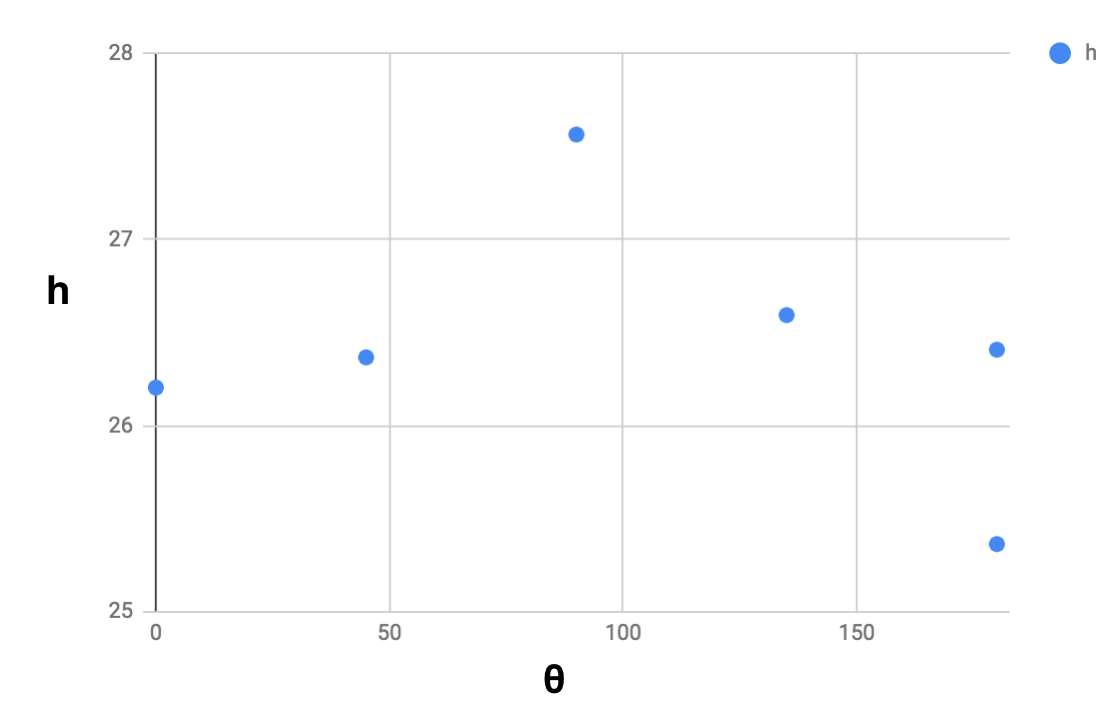
\includegraphics[width=7cm]{../img/htheta.png}
        \caption{$h\ \sim \ \theta$の関係}
      \end{center}
    \end{figure}
  \item (2),(4)の導出
    \begin{enumerate}
      \item (2) \\
        $Q_{x} = - S(k \frac{dT}{dx})$ \\
        $Q_{x+dx} = -S \{ k \frac{dT}{dx} + \frac{d}{dx} (k\frac{dT}{dx})dx     \}        $ \\
        $\frac{dQ_{x}}{dx} - \frac{dQ_{x+dx}}{dx} - \frac{dQ_{f}}{dx}$ \\
        より,(2)が導かれる.

      \item (4)
        (3)を解くと(4)が得られる.
    \end{enumerate}
  
  \item 自然対流時の$\theta = 90 \circ$の時の放熱量$Q$ \\
    $\theta = 90 \circ$の時,$Q = 5.399J$,$Q_{N} = 8.83J$との差が安定するまで測定を行なった.
    \par また,$IE = 3.43$となった.
    \par $\frac{NQ}{IE} = 2.56$より,$Q_{N}$の方が2.56倍
    $IE$よりも大きかった.
    \par これは,(9)より近似式を用いており,$A_{w}$はフィン表面
    以外での流体との接触面積を指しているが,これはフィンと空気との
    接触面積に比べて小さいことを用いて近似をしている.しかし,
    1枚からの放出熱が付近の他のフィンを温めてしまうため,$NQ$の方が2.56
    倍も高くなったと考えられた.
  \item $\theta$と$h$の関係 \\
    空気は温まると上昇する性質があり,同様に様々な$\theta$の値で本実験でもその現象が起こり,ヒータ付近で
    温められた気体が上昇し,上部で冷えたのち下降して対流が発生したからと
    考えられる.
  \item 強制対流時の熱伝達率と同じ姿勢における自然対流時の熱伝達率 \\
    $\theta = 180 \circ$の時,表2よりファンをつけた時の方が$h$が大きくなっている.
    強制対流によって温まった空気が風に流されたことにより,熱伝達率も上がったと
    考えられる.
    効率的な放熱促進処置としては,ファンをフィンの方向に向けて冷却するという手段が
    考えられた.
  \item 計測技術の適用方法
    本実験では熱電対を用いた.これは,接触式の温度センサーで2種類の異なる金属を
    接続し,各接点間の起電力を利用して温度を計測するセンサーである.
    熱電対は安価に入手でき構造が単純なため高い信頼性を得ることができる.
    また,広範囲の温度の測定も可能である.素線を用いることで,
    応答速度の向上が得られたり,部分的な温度,高圧下や真空雰囲気における温度を
    測定することができる.
    \par また,非接触式の温度センサーもあり,小物体,動く物体,近づけない物体
    などの温度を測定できるが,接触式に比べ精度は劣る.
    
\end{enumerate}

% 結果
\begin{thebibliography}{1}
  \bibitem{}知能機械工学基礎実験テキスト P.106-P.110
  \bibitem{}株式会社キーエンス,放射温度計の基礎 https://www.keyence.co.jp/ss/products/recorder/lab/thermometry/radiation.jsp
  \bibitem{}石川産業株式会社 http://www.ishikawa-sangyo.co.jp/thermocouples/wire/index.html
\end{thebibliography}
\end{document}